\let\negmedspace\undefined
\let\negthickspace\undefined
\documentclass[journal]{IEEEtran}
\usepackage[a5paper, margin=10mm, onecolumn]{geometry}
\usepackage{lmodern} % Ensure lmodern is loaded for pdflatex
\usepackage{tfrupee} % Include tfrupee package

\setlength{\headheight}{1cm} % Set the height of the header box
\setlength{\headsep}{0mm}     % Set the distance between the header box and the top of the text

\usepackage{gvv-book}
\usepackage{gvv}
\usepackage{cite}
\usepackage{amsmath,amssymb,amsfonts,amsthm}
\usepackage{algorithmic}
\usepackage{graphicx}
\usepackage{textcomp}
\usepackage{xcolor}
\usepackage{txfonts}
\usepackage{listings}
\usepackage{enumitem}
\usepackage{mathtools}
\usepackage{gensymb}
\usepackage{comment}
\usepackage[breaklinks=true]{hyperref}
\usepackage{tkz-euclide} 
\usepackage{listings}
 \usepackage{gvv}                                        
\def\inputGnumericTable{}                                 
\usepackage[latin1]{inputenc}                                
\usepackage{color}                                            
\usepackage{array}                                            
\usepackage{longtable}                                       
\usepackage{calc}                                             
\usepackage{multirow}                                         
\usepackage{hhline}                                           
\usepackage{ifthen}                                           
\usepackage{lscape}
\begin{document}

\bibliographystyle{IEEEtran}


\title{2.10.50}
\author{EE25BTECH11021 - Dhanush Sagar
}
% \maketitle
% \newpage
% \bigskip
{\let\newpage\relax\maketitle}

\renewcommand{\thefigure}{\theenumi}
\renewcommand{\thetable}{\theenumi}
\setlength{\intextsep}{10pt} % Space between text and floats
\numberwithin{equation}{enumi}
\numberwithin{figure}{enumi}
\renewcommand{\thetable}{\theenumi}
\textbf{Question} \\
Find the equation of the line passing through (1, 2) and making angle 30\degree with y-axis.\\

\textbf{Solution:} \\[6pt]
Given point,
\begin{align}
 \vec{A} = \myvec{1 \\ 2}
\end{align}
and the line makes an angle of $30^\circ$ with the y-axis. \\[6pt]

The slope of the line is reciprocal of $\tan 30^\circ$:  
\begin{align}
m &= \frac{1}{\tan 30^\circ}
\end{align}

Evaluating, we get:  
\begin{align}
m &= \sqrt{3}
\end{align}

The direction vector of the line is $\myvec{1 \\ m}$, hence the normal vector is:  
\begin{align}
\Vec{n} &= \myvec{\sqrt{3} \\ -1}
\end{align}

Equation of the line is given by :  
\begin{align}
\Vec{n}^\top \vec{x} &=\Vec{n}^\top \vec{A}
\end{align}

Substituting the values of $\vec{n}$ and $\vec{A}$:  
\begin{align}
\myvec{\sqrt{3} & -1} \vec{x} &= \myvec{\sqrt{3} & -1}\myvec{1 \\ 2}
\end{align}

Evaluating the RHS gives:  
\begin{align}
\myvec{\sqrt{3} & -1} \vec{x} &= \sqrt{3} - 2
\end{align}
\begin{figure}[H]
    \centering
    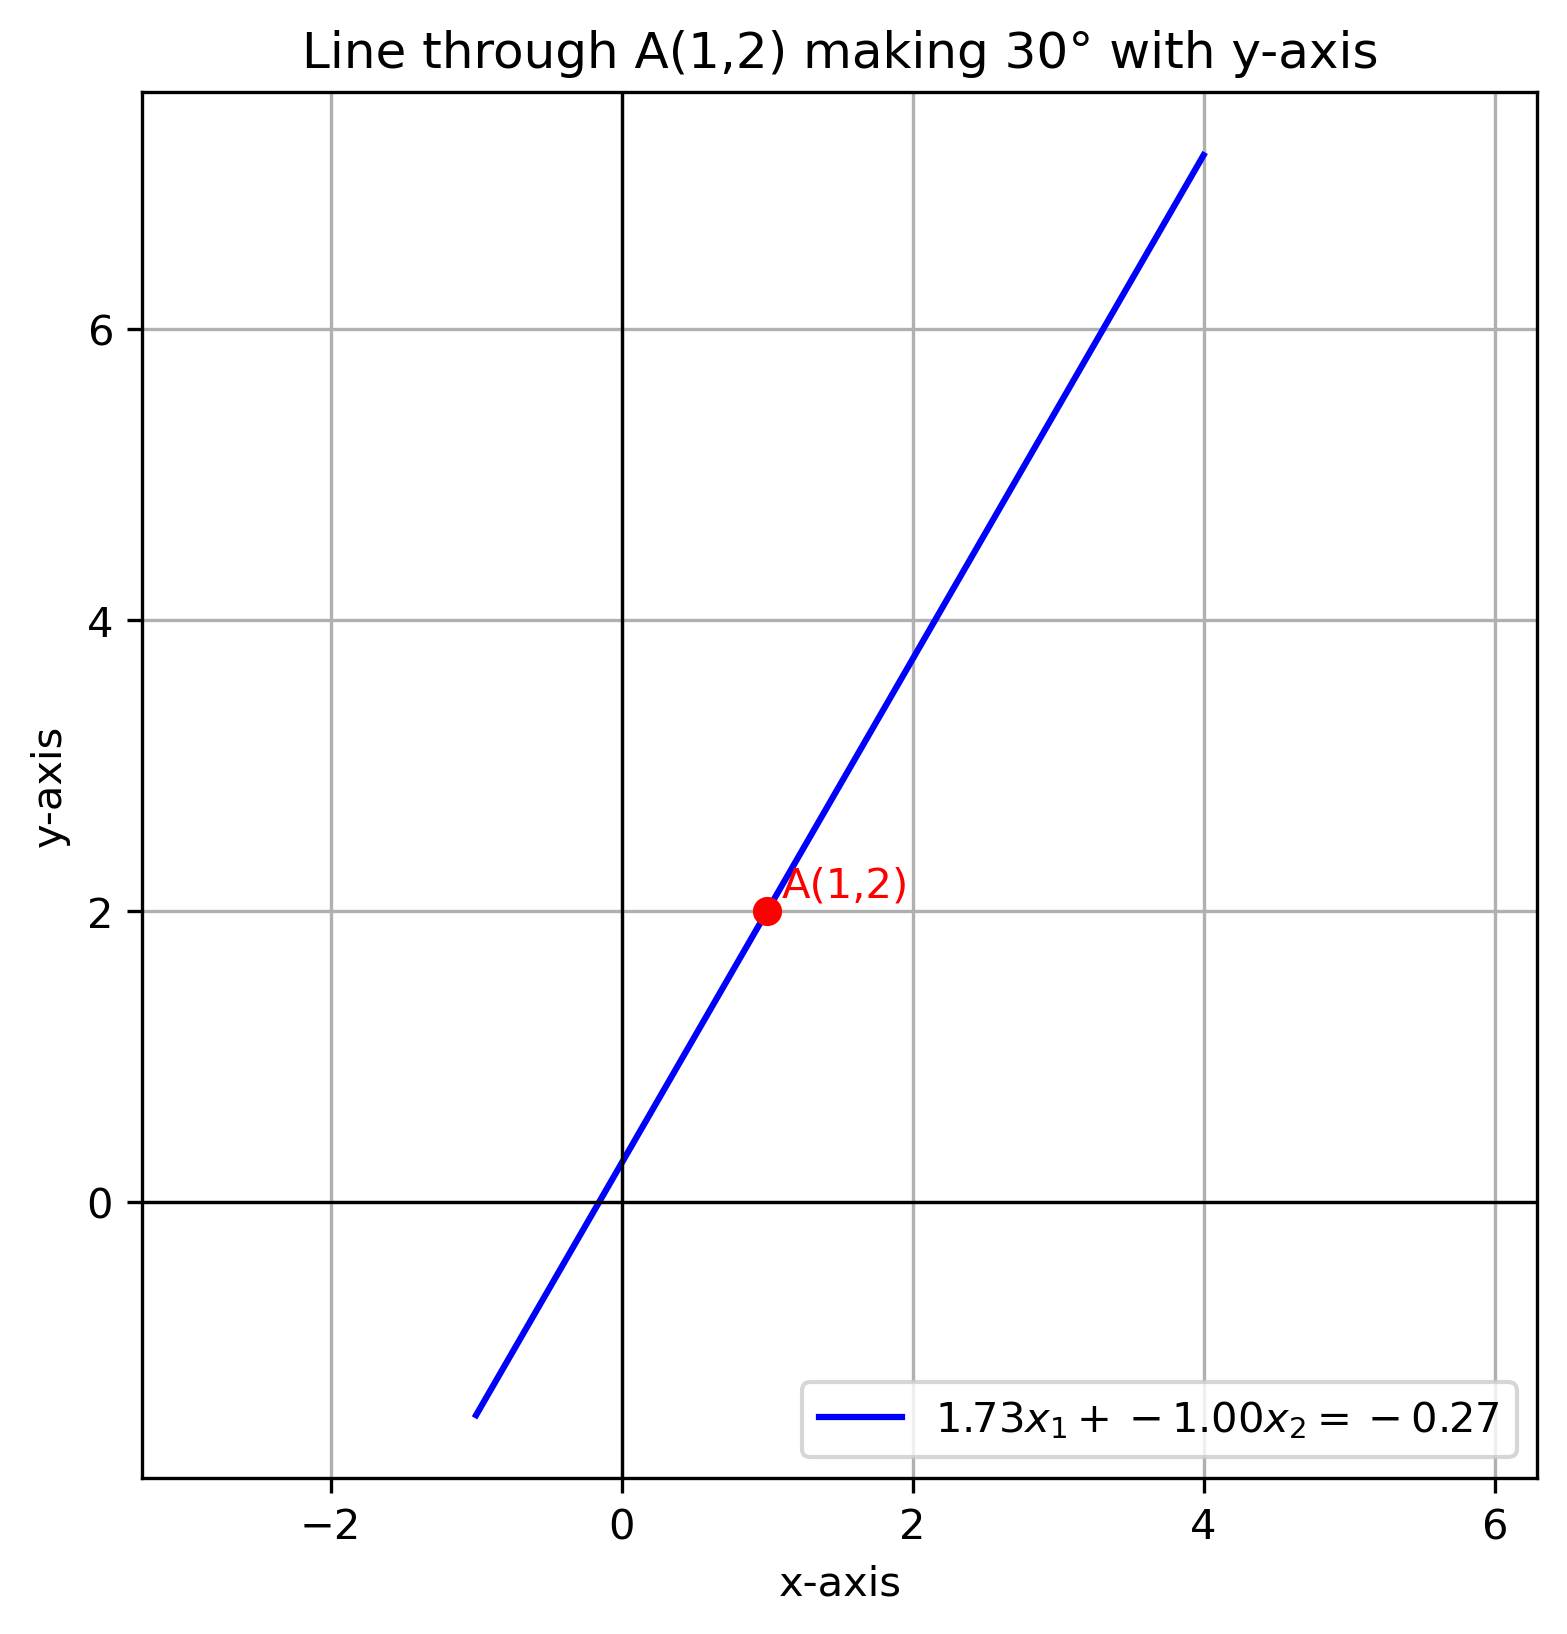
\includegraphics[width=0.5\columnwidth]{figs/fig1.png}
    \caption{}
    \label{fig:placeholder}
\end{figure}

\end{document}